The design approach described in this article is not intended to
replace sound engineering of an intelligent system, but rather as 
an additional step that may be applied to a system in order to provide
the system with more agility, flexibility, and the ability to be rapidly
re-tasked. As such, it is assumed that a system has been implemented
that is capable of basic robotic actions. In our case, our knowledge
driven system bottoms out in a Robot Operating System (ROS) control layer
\footnote{Certain commercial/open source software and tools are identified 
in this paper in order to explain our research. Such identification does not imply
recommendation or endorsement by the authors or NIST, nor does it 
imply that the software tools identified are necessarily the best available for the purpose.}.
\begin{figure}[ht!]
\begin{center}
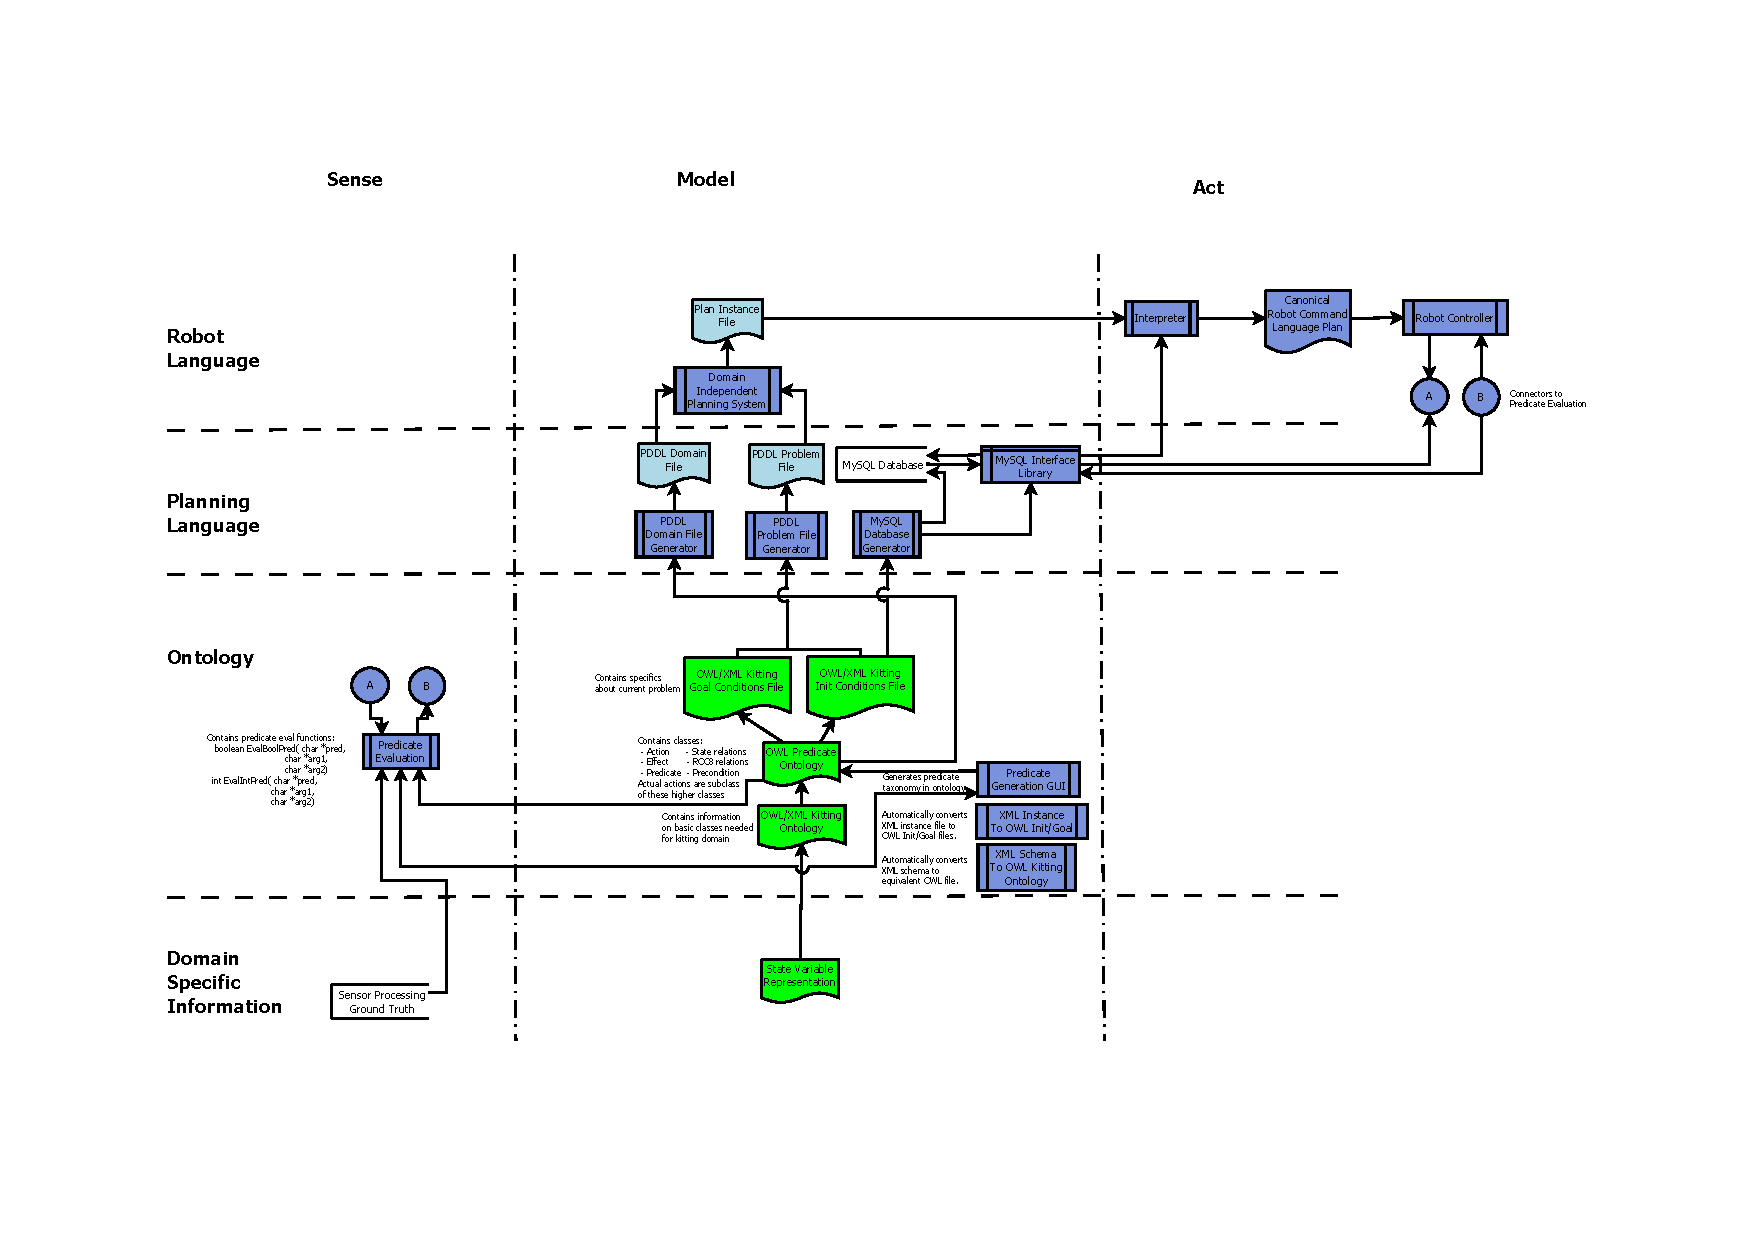
\includegraphics[width=16cm]{images/KnowledgeDrivenRobotics.pdf}
\caption{Knowledge Driven Design extensions.}
\label{fig:DesignArchitecture}
\end{center}
\end{figure}

The overall architecture of the system may be seen in Figure \ref{fig:DesignArchitecture}.
The design begins with requirements generation from a domain expert. 
A very systematic scenario driven approach for identifying and 
modeling the concepts has been taken. A scenario 
was developed that described, in detail, the types of operations that would be performed 
in the target application, the sequencing of steps, the parts and machines that were 
needed, constraints 
on the process such as pre- and post-conditions, etc. For this scenario, a set of 
concepts were extracted and defined. These concepts served as the initial requirements 
for the knowledge that must be encoded for the domain.
This knowledge was encoded in the form of a state variable representation (SVR). 
In a SVR, each state is represented by a tuple of values of $n$ state variables 
$\lbrace x_1,\dots,x_n\rbrace$, and each action is represented by a partial function 
that maps this tuple into some other tuple of values of the $n$ state variables.
The concepts that were modeled in the SVR, built off of the 
definitions and relationships that were identified in the scenario. 

The design transitions from domain expertise to knowledge modeling expertise
when the SVR is used to generate an ontology which consists of a base ontology
that describes the objects in the scenario, extensions that describe the
actions and predicates relevant to the scenario, and instance files that
describe the initial and goal states for the system. The ontology files are
described in more detail in Section \ref{Sect:Ontology}.

From this point forward, automatic planning tools have been designed to transition 
the knowledge into a planning framework and finally a robot specific framework.

